\begin{figure*}[t!]
    \centering
    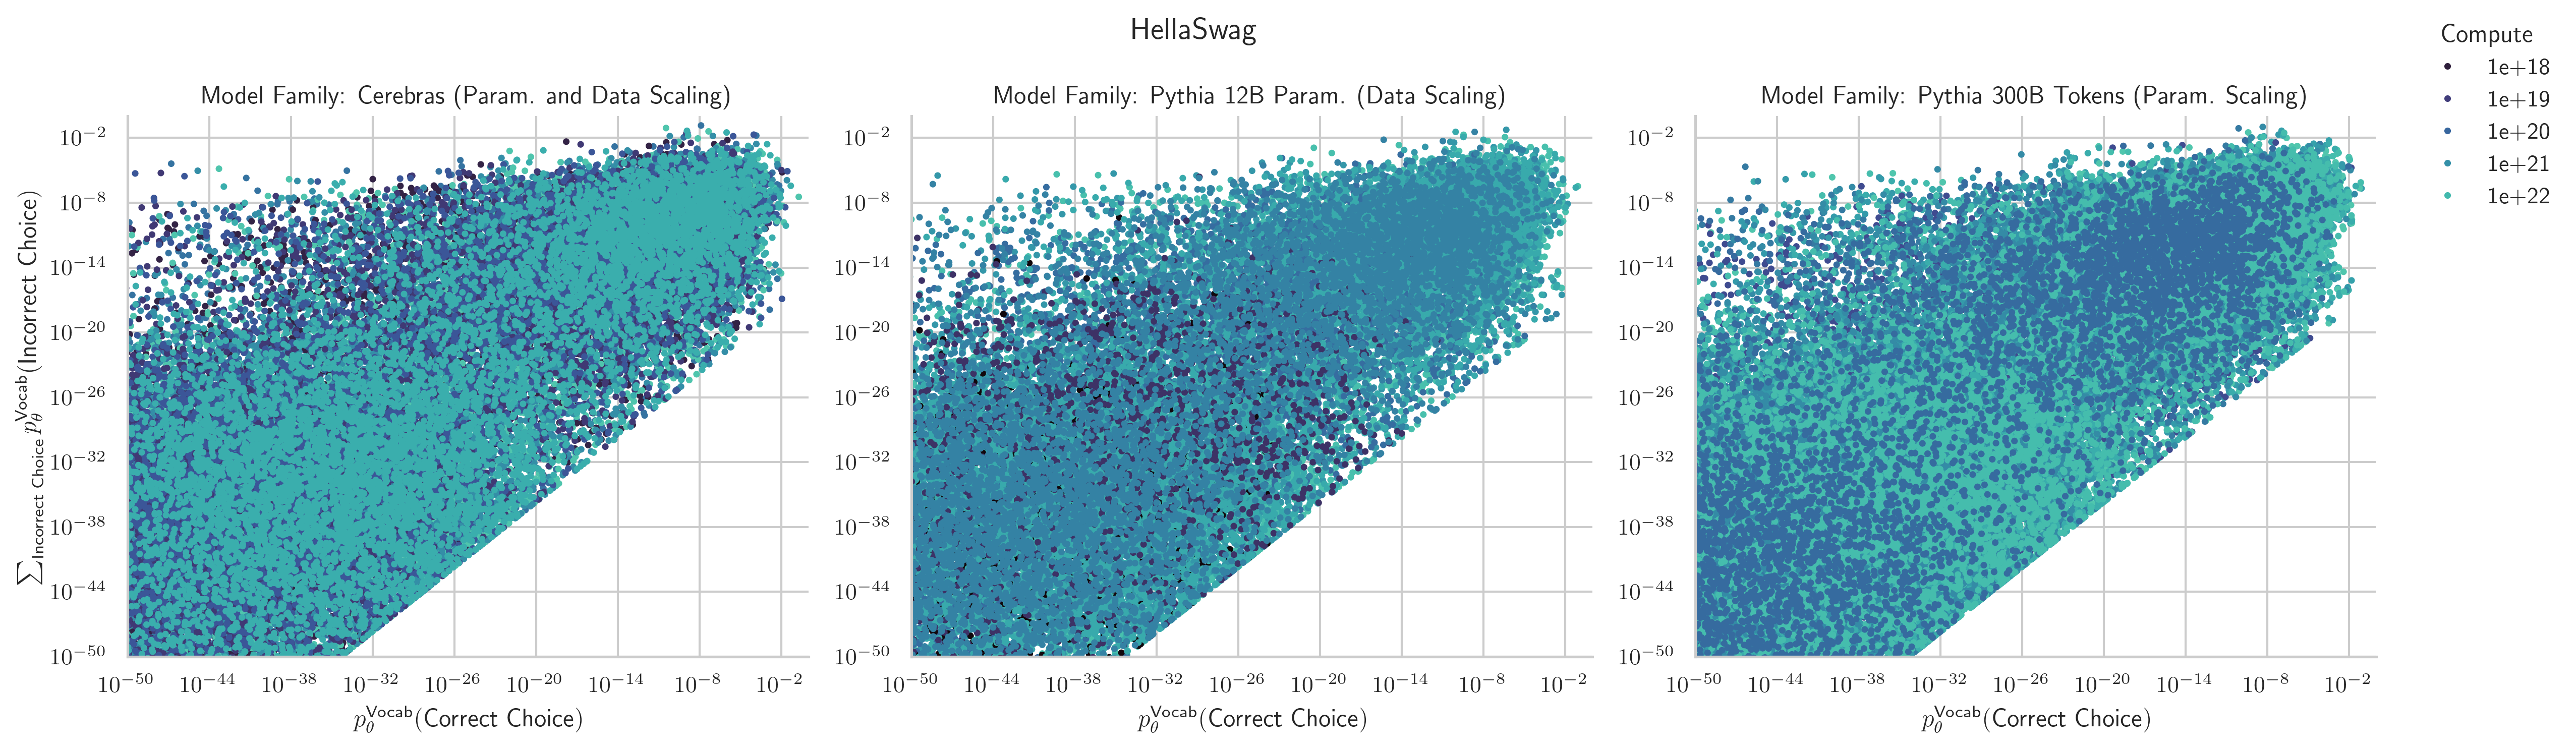
\includegraphics[width=\textwidth]{figures/pvocab_correct_vs_pvocab_incorrect/hellaswag/hellaswag_prob_other_choices_vocab_vs_prob_correct_vocab_scatter_by_compute_split_model_family.png}
    % 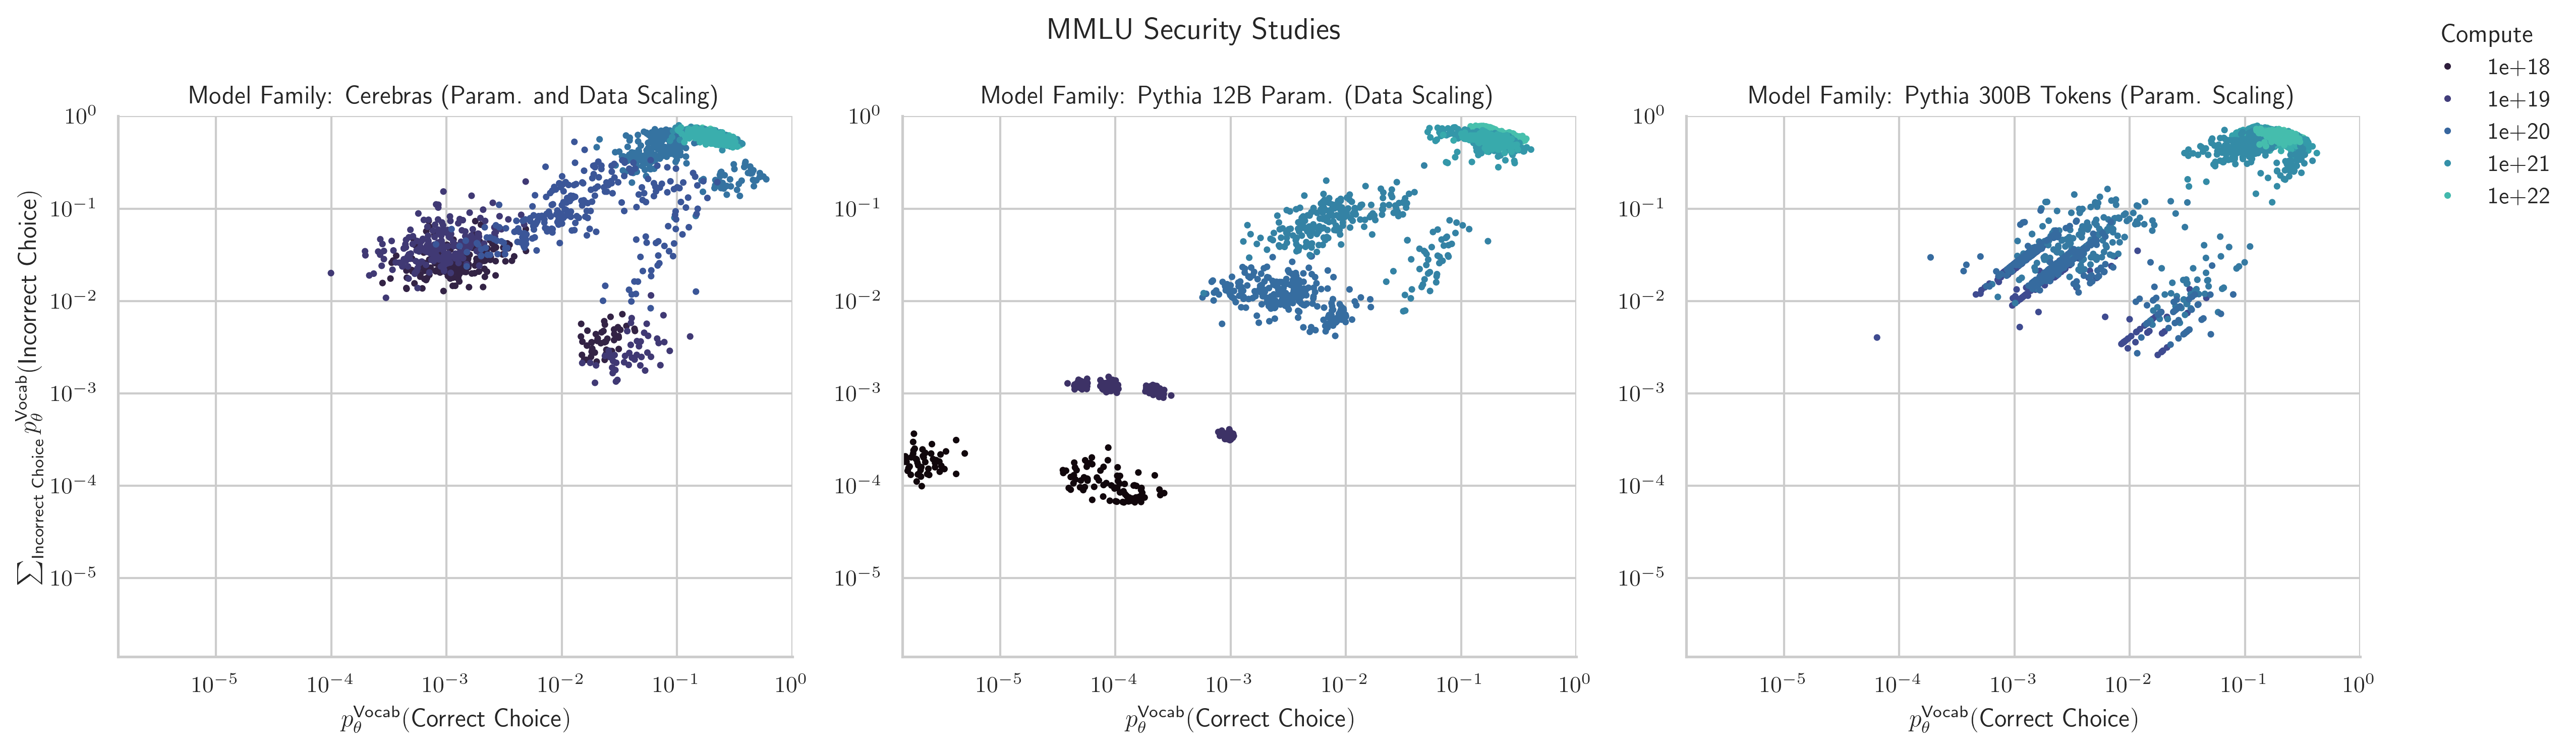
\includegraphics[width=\textwidth]{figures/pvocab_correct_vs_pvocab_incorrect/mmlu_security_studies/mmlu_security_studies_prob_other_choices_vocab_vs_prob_correct_vocab_scatter_by_compute_split_model_family.png}
    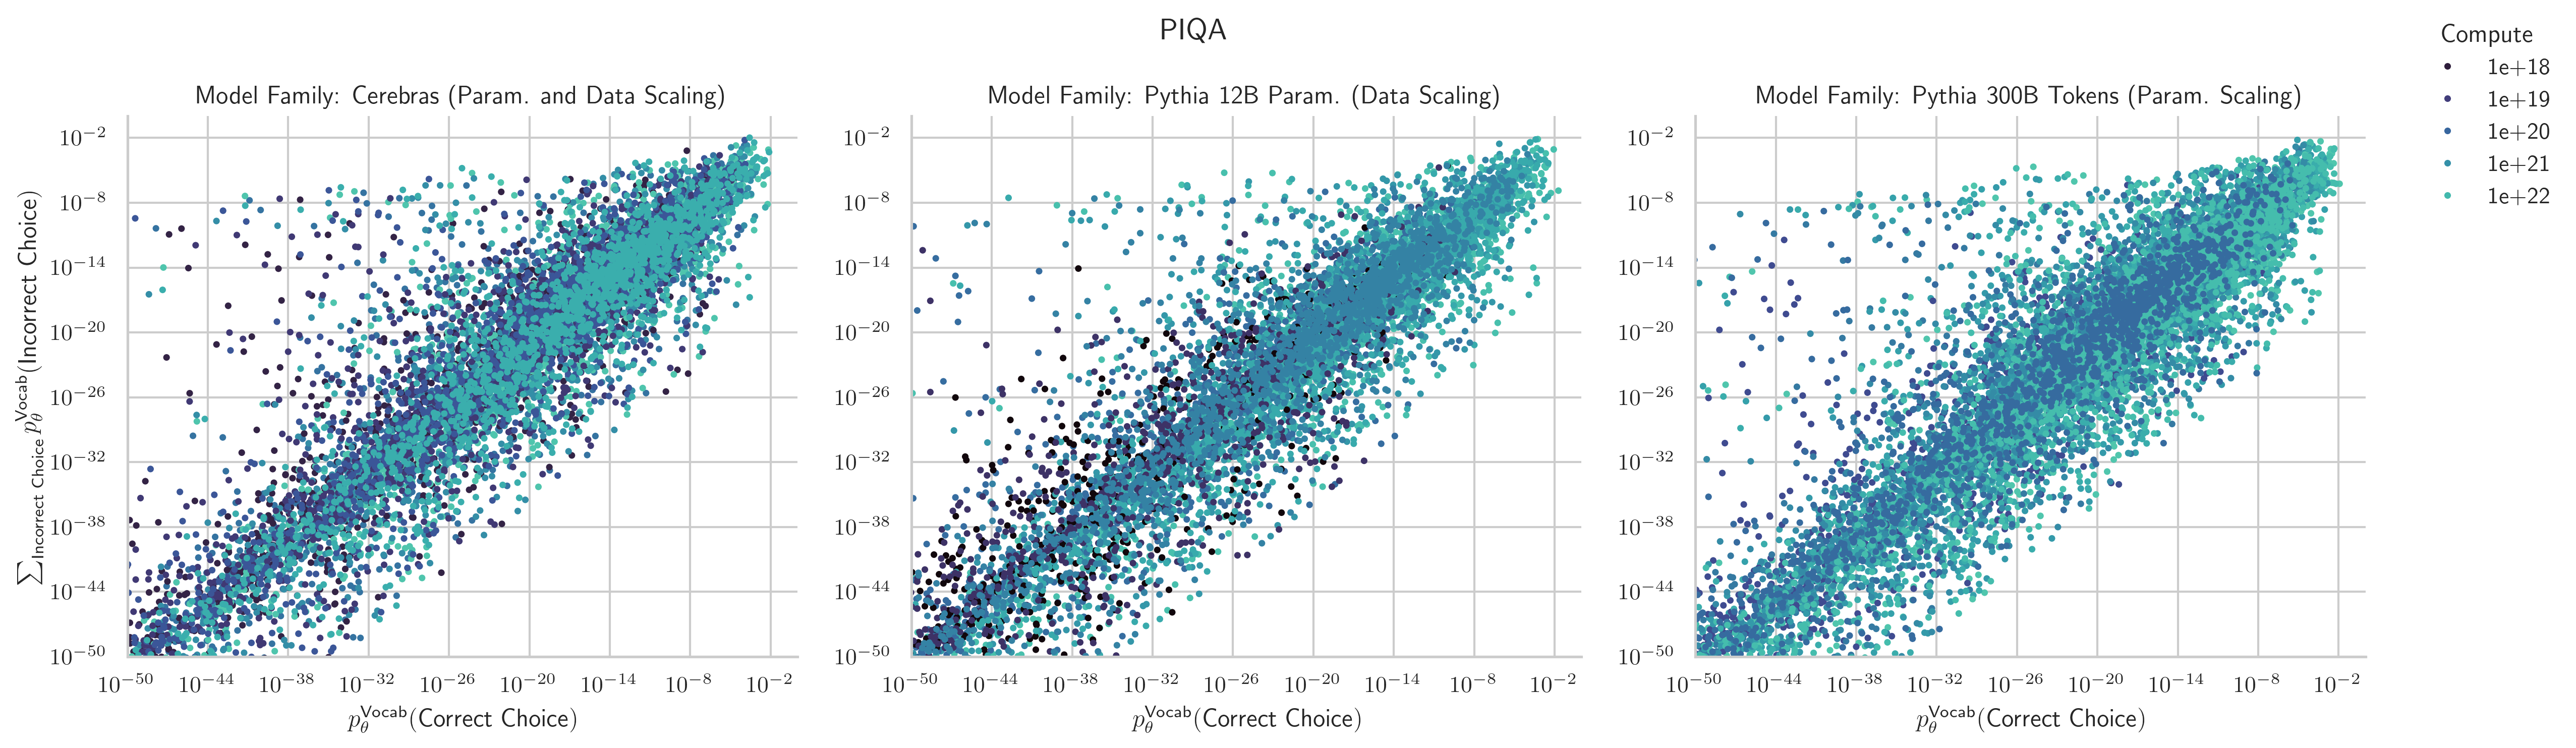
\includegraphics[width=\textwidth]{figures/pvocab_correct_vs_pvocab_incorrect/piqa/piqa_prob_other_choices_vocab_vs_prob_correct_vocab_scatter_by_compute_split_model_family.png}
    \caption{\textbf{Probability mass on the correct choices and the incorrect choices are correlated, but can fluctuate substantially.} Probability mass on correct choices and incorrect choices positively covaries and typically increases with compute. However, the spread is large: for any given value of $p^{\text{Vocab}}_{\theta} (\text{Correct Choice})$, the mass on incorrect choices can vary by many orders of magnitude.}
    \label{fig:pvocab_correct_vs_pvocab_incorrect}
\end{figure*}

\section{Scaling Behavior of Probability Mass on Incorrect Choices}

In general, aggregate performance over a distribution is often of interest. Such a focus on aggregate performance leads to an important insight: in MCQA, probability mass fluctuations on incorrect choices do not ``average out". Unlike estimating the mean of a random variable, where positive and negative deviations cancel, the nonlinear nature of metrics like Accuracy and Brier Score means that probability mass shifts between incorrect options affect scores in complex ways that persist under averaging. For example, if probability mass shifts from incorrect option A to incorrect option B, the impact on accuracy depends on whether either option had enough mass to compete with the correct answer - there's no natural cancellation. This perhaps counter-intuitive behavior partially explains why predicting aggregate performance via averaging has remained elusive.

This analysis suggests that modeling probability mass fluctuations on incorrect choices could improve predictions of metrics like Accuracy and Brier Score, though the magnitude of improvement remains an open question.
For metrics like $\texttt{Accuracy}$, such predictions should be made for each sample because knowing the average mass (across many data) placed on incorrect choices says little about how much mass is placed on any single incorrect choice for a single sample.
We conclude by providing preliminary evidence that achieving such a feat might be possible. Specifically, we test how probability masses on correct choices and probability masses on incorrect choices covary with increasing compute (Fig. \ref{fig:pvocab_correct_vs_pvocab_incorrect}). Multiple benchmarks display strong positive relationships between mass on correct choices and mass on incorrect choices, suggesting that fitting \textit{per-sample scaling trends for each incorrect choice} might be possible; doing so might enable better predicting changepoints in metrics like \texttt{Accuracy} or \texttt{Brier Score}. However, whether per-benchmark per-sample per-choice scaling trends can be fit and accurately extrapolated is unclear since the spread varies by several orders of magnitude. We leave this challenge to future work.
